\section{Durchführung}
\label{sec:Durchführung}

Für die vier durchzuführenden Messungen werden die Schaltplänge gemäß
Abbildung \ref{fig:Aufbau} verwendet. Hierbei ist zu beachten, dass statt eines 
Nadelimpulses ein Rechtecksignal benutzt wird. 

\begin{figure}
  \centering
  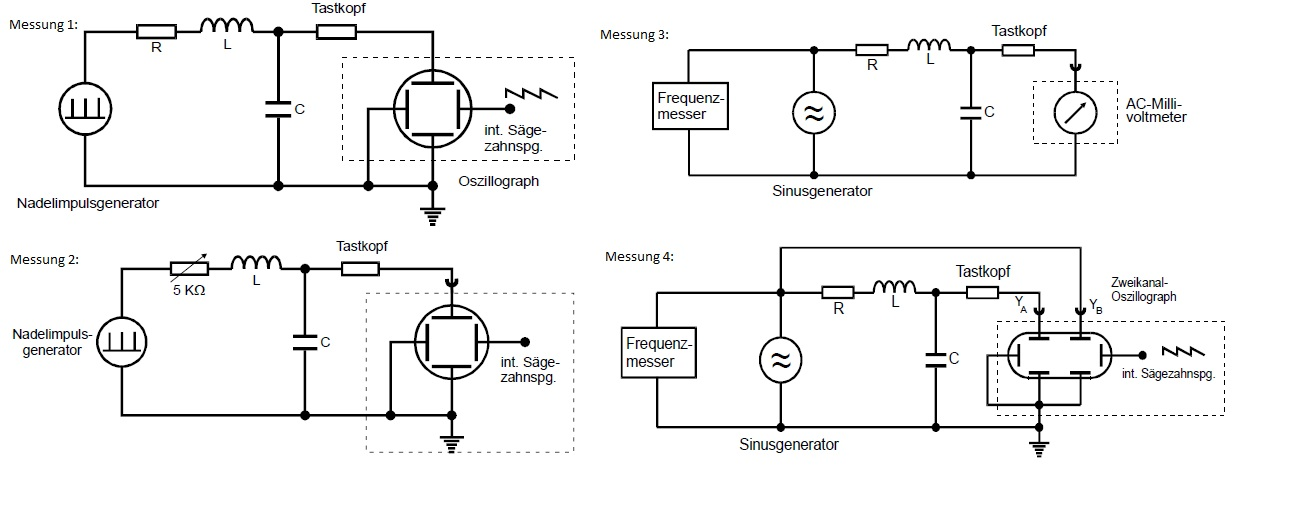
\includegraphics[scale=0.4]{content/Aufbau_Schaltungen.jpg}
  \caption{Die vier verwendeten Schaltungen}
  \label{fig:Aufbau}
\end{figure}

Zunächst werden die bauteilspezifischen Werte, wie Kapazität $C$
und Induktivität $L$ notiert. 

Im ersten Versuchsteil wird ein RLC-Kreis mit niederfrequenten 
Rechteckimpulsen ausgelenkt und so zum Schwingen angeregt. Nach Abfall
eines Rechteckimpulses wird der zeitliche Verlauf der Kondensatorspannung
gemessen. Die so entstehende gedämpfte Schwingung wird mit Hilfe eines
Oszilloskops aufgezeichnet und gespeichert. 

Bei dem zweitem Versuchsteil wird der zuvor feste Widerstand durch einen 
regelbaren Widerstand, ein Potentiometer, ersetzt. Dieser wird so eingestellt, 
dass der aperiodische Grenzfall vorliegt, es also gerade zu keiner Schwingung des 
Sytems mehr kommt. Der dazugehörige Wert für $R$ wird notiert. Auch diese 
entstehende Kurve des Spannungsabfalls wird mit dem Oszilloskops aufgezeichnet 
und gespeichert. 

Im drittem Versuchsteil wird die Kondensatorspannung in Abhängigkeit von 
der Frequenz einer anliegenden Sinusspannung untersucht. Die Frequenz
liegt dabei in einem Bereich von 1-$\SI{64.5}{\kilo\hertz}$. 

Die letzte Messung untersucht die im drittem Versuchsteil entstehende 
Phasenverschiebung zwischen der Kondensator- und Sinusspannung. Gemessen 
wird diese durch den Vergleich der beiden Spannungen auf dem Oszilloskop. 


